\section{Feature Engineering for Clustering}
\label{sec:feat_eng}
In this phase, we focused on creating features specifically for the cyclist dataset, as the subsequent clustering step was performed exclusively on this data. However, the race dataset was also essential for calculating these features, as the new cyclist features were derived from their career performance. Initially, features were also created specifically for the race dataset during an exploratory phase, but these were ultimately not used since the decision to cluster only on the cyclist dataset was made later.
To focus the analysis on professional cyclists, we selected those with more than 20 races to date. This filtering was done before the feature engineering step to not alter the distributions of the engineered features.

\subsection{Engineered Features Overview}

\noindent
\textbf{cyclist\_experience:} counts how many stages the cyclist participates in as an overall experience.\\

\noindent
\textbf{cyclist\_experience\_points:} It represents the total points accumulated by each cyclist in the races they participated in (not weighted by position). \\

\noindent
\textbf{cyclist\_win:}
count how many stages are won by each cyclist.\\

\noindent
\textbf{cyclist\_win\_ratio:} compute the ratio between stages won and stages in which the cyclist participated. \\

\noindent
\textbf{avg\_position:} it is the average position considering all the races the cyclist has participated in.\\

\noindent
\textbf{avg\_relative\_position:} This feature represents the average placement of a cyclist throughout their career, with each position normalized according to the number of participants in each race.\\

\noindent
\textbf{min\_relative\_position:} it is the best (minimum) relative position achieved by a cyclist.\\

\noindent
\textbf{relative\_position\_std:} this feature highlights a cyclist's performance consistency: a low standard deviation indicates steady results, while a high standard deviation reflects variability influenced by factors like race difficulty or participant numbers or weather conditions, etc.\\

\noindent
\textbf{best\_position:} it is the best (minimum) position achieved by a cyclist.\\

\noindent
\textbf{position\_std:} It's like \textit{relative\_position\_std} but the position is not normalized by the number of cyclists.\\

\noindent
\textbf{mean\_last\_20\_positions:} This feature represents the average position achieved in the 20 worst performances of a cyclist.\\

\noindent
\textbf{mean\_last\_20\_positions\_1:} This feature is similar to the previous one, but the worst placements are selected based on relative ranking rather than solely considering absolute position when identifying the 20 worst performances. \\

\noindent
\textbf{avg\_position\_vs\_startlist}: the average relative position achieved by a cyclist, normalized by the start list quality to account for race difficulty.\\

\noindent
\textbf{performance\_entropy:} It's a performance variability metric. It measures the consistency of a cyclist's performance across races. Lower values indicate consistent results, while higher values reflect more fluctuating performance, similar to position standard deviation.\\

\noindent
\textbf{weighted\_podiums:} 
The value of the feature is calculated as follows:
\[
\text{Weighted Podium}_{j} =  \frac{1}{T_j}  \sum_{r=1}^{R} \left( w_i \cdot point_{r} \cdot N_r \right)
\]

\noindent
with \( r \) representing a specific race, ranging from 1 to \( R \), which is the total number of races. The variable \( w_i \) denotes the weight assigned to a cyclist's position ($w_1$ for first place, $w_2$ for second place, $w_3$ for third place, 0 otherwise). The points awarded for a race \( r \) are represented as \( point_r \). \( N_r \) is the total number of cyclists participating in race \( r \), while \( T_j \) indicates the total number of races completed by cyclist \( j \).\\


\noindent
\textbf{career\_level:} 
This feature represents the level of a cyclist by summing all the placements achieved in their career, weighted by the points of the races and considering the placements reached in their career, taking into account the points of the races they participated in and the number of cyclists in those races:
\[
\text{Career Level}_j = \sum_{r=1}^{R_j} \frac{(\text{N}_r - \text{pos}_{j,r}) \cdot \text{points}_r}{\text{N}_r}
\]

\noindent
\( r \) represents a specific race, ranging from 1 to \( R \) (the total number of races). The variable \(\text{pos}_{j,r}\) indicates the position of cyclist \( j \) in race \( r \). The points awarded for race \( r \) are represented as \(\text{points}_r\), and \( N_r \) refers to the total number of cyclists participating in race \( r \).\\

\noindent
\textbf{mean\_sq:} it represents the average start list quality of all the races the cyclist participated in. This feature represents somehow the "relevance" but also "the difficulty" on average of the stages in which a cyclist participated. \\

\noindent
\textbf{top\_cyclists:} this feature is calculated by dividing cyclists into ranked segments based on the ordered values of the \textit{career\_level} feature, such as top 10, top 20, and so on.\\

\noindent
\textbf{top\_experience:} it is calculated by dividing cyclists into ranked segments based on the ordered values of the \textit{cyclist\_experience} feature, such as top 10, top 20, and so on, to somehow categorize cyclists based on their experience. \\


\begin{figure}[H]
\centering
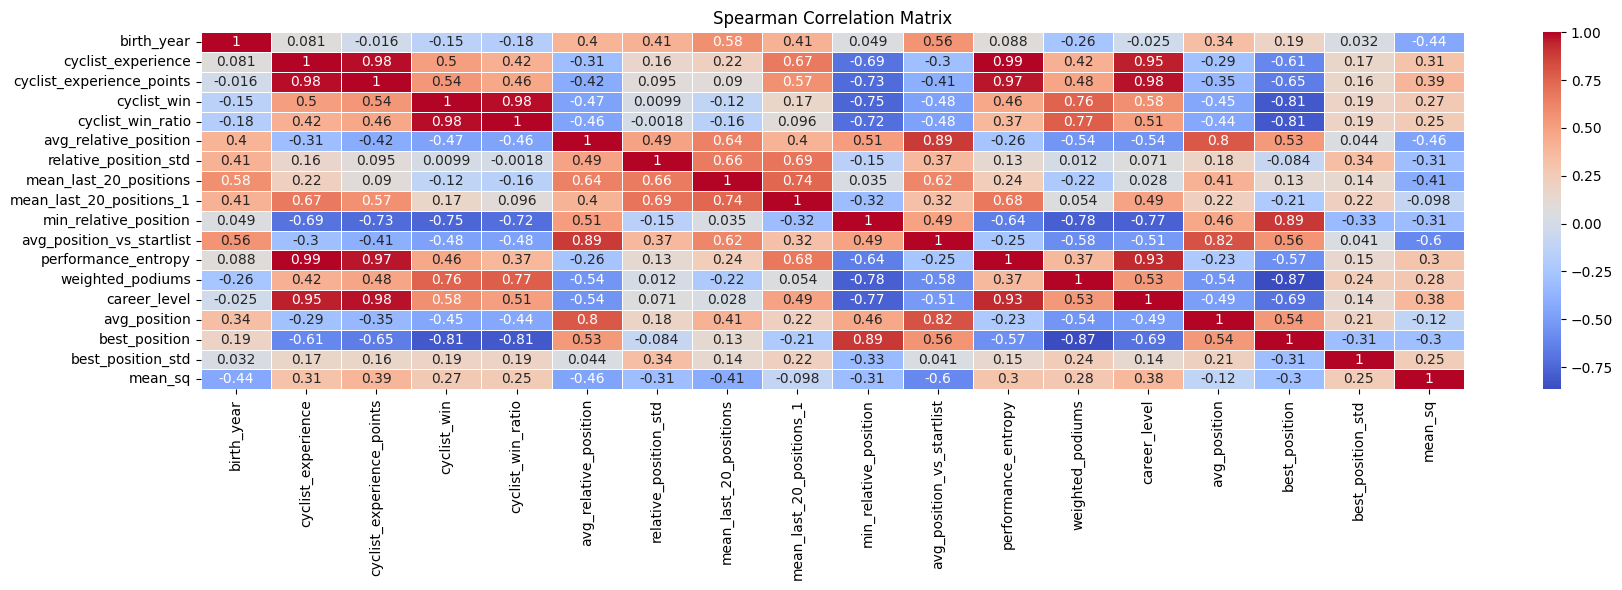
\includegraphics[width=1\textwidth]{images/DE/correlation.png}
\caption{\small Spearman Correlation Analysis on Cyclist Dataset}
\label{fig:cyclists_feature_correlation}
\end{figure}

\subsection{Correlation}

\autoref{fig:cyclists_feature_correlation} presents a correlation plot of the engineered features. While Kendall-based correlations are also available in the notebook, we chose to focus on Spearman correlations. Spearman correlations often exhibit similar trends but yield higher values, treating features as more correlated. This makes them more suitable for the next clustering step, where it is important to select features with limited correlation.

